% Options for packages loaded elsewhere
\PassOptionsToPackage{unicode}{hyperref}
\PassOptionsToPackage{hyphens}{url}
\documentclass[
  12pt,
]{article}
\usepackage{xcolor}
\usepackage[margin=1in]{geometry}
\usepackage{amsmath,amssymb}
\setcounter{secnumdepth}{-\maxdimen} % remove section numbering
\usepackage{iftex}
\ifPDFTeX
  \usepackage[T1]{fontenc}
  \usepackage[utf8]{inputenc}
  \usepackage{textcomp} % provide euro and other symbols
\else % if luatex or xetex
  \usepackage{unicode-math} % this also loads fontspec
  \defaultfontfeatures{Scale=MatchLowercase}
  \defaultfontfeatures[\rmfamily]{Ligatures=TeX,Scale=1}
\fi
\usepackage{lmodern}
\ifPDFTeX\else
  % xetex/luatex font selection
  \setmainfont[]{Times New Roman}
\fi
% Use upquote if available, for straight quotes in verbatim environments
\IfFileExists{upquote.sty}{\usepackage{upquote}}{}
\IfFileExists{microtype.sty}{% use microtype if available
  \usepackage[]{microtype}
  \UseMicrotypeSet[protrusion]{basicmath} % disable protrusion for tt fonts
}{}
\makeatletter
\@ifundefined{KOMAClassName}{% if non-KOMA class
  \IfFileExists{parskip.sty}{%
    \usepackage{parskip}
  }{% else
    \setlength{\parindent}{0pt}
    \setlength{\parskip}{6pt plus 2pt minus 1pt}}
}{% if KOMA class
  \KOMAoptions{parskip=half}}
\makeatother
\usepackage{color}
\usepackage{fancyvrb}
\newcommand{\VerbBar}{|}
\newcommand{\VERB}{\Verb[commandchars=\\\{\}]}
\DefineVerbatimEnvironment{Highlighting}{Verbatim}{commandchars=\\\{\}}
% Add ',fontsize=\small' for more characters per line
\usepackage{framed}
\definecolor{shadecolor}{RGB}{248,248,248}
\newenvironment{Shaded}{\begin{snugshade}}{\end{snugshade}}
\newcommand{\AlertTok}[1]{\textcolor[rgb]{0.94,0.16,0.16}{#1}}
\newcommand{\AnnotationTok}[1]{\textcolor[rgb]{0.56,0.35,0.01}{\textbf{\textit{#1}}}}
\newcommand{\AttributeTok}[1]{\textcolor[rgb]{0.13,0.29,0.53}{#1}}
\newcommand{\BaseNTok}[1]{\textcolor[rgb]{0.00,0.00,0.81}{#1}}
\newcommand{\BuiltInTok}[1]{#1}
\newcommand{\CharTok}[1]{\textcolor[rgb]{0.31,0.60,0.02}{#1}}
\newcommand{\CommentTok}[1]{\textcolor[rgb]{0.56,0.35,0.01}{\textit{#1}}}
\newcommand{\CommentVarTok}[1]{\textcolor[rgb]{0.56,0.35,0.01}{\textbf{\textit{#1}}}}
\newcommand{\ConstantTok}[1]{\textcolor[rgb]{0.56,0.35,0.01}{#1}}
\newcommand{\ControlFlowTok}[1]{\textcolor[rgb]{0.13,0.29,0.53}{\textbf{#1}}}
\newcommand{\DataTypeTok}[1]{\textcolor[rgb]{0.13,0.29,0.53}{#1}}
\newcommand{\DecValTok}[1]{\textcolor[rgb]{0.00,0.00,0.81}{#1}}
\newcommand{\DocumentationTok}[1]{\textcolor[rgb]{0.56,0.35,0.01}{\textbf{\textit{#1}}}}
\newcommand{\ErrorTok}[1]{\textcolor[rgb]{0.64,0.00,0.00}{\textbf{#1}}}
\newcommand{\ExtensionTok}[1]{#1}
\newcommand{\FloatTok}[1]{\textcolor[rgb]{0.00,0.00,0.81}{#1}}
\newcommand{\FunctionTok}[1]{\textcolor[rgb]{0.13,0.29,0.53}{\textbf{#1}}}
\newcommand{\ImportTok}[1]{#1}
\newcommand{\InformationTok}[1]{\textcolor[rgb]{0.56,0.35,0.01}{\textbf{\textit{#1}}}}
\newcommand{\KeywordTok}[1]{\textcolor[rgb]{0.13,0.29,0.53}{\textbf{#1}}}
\newcommand{\NormalTok}[1]{#1}
\newcommand{\OperatorTok}[1]{\textcolor[rgb]{0.81,0.36,0.00}{\textbf{#1}}}
\newcommand{\OtherTok}[1]{\textcolor[rgb]{0.56,0.35,0.01}{#1}}
\newcommand{\PreprocessorTok}[1]{\textcolor[rgb]{0.56,0.35,0.01}{\textit{#1}}}
\newcommand{\RegionMarkerTok}[1]{#1}
\newcommand{\SpecialCharTok}[1]{\textcolor[rgb]{0.81,0.36,0.00}{\textbf{#1}}}
\newcommand{\SpecialStringTok}[1]{\textcolor[rgb]{0.31,0.60,0.02}{#1}}
\newcommand{\StringTok}[1]{\textcolor[rgb]{0.31,0.60,0.02}{#1}}
\newcommand{\VariableTok}[1]{\textcolor[rgb]{0.00,0.00,0.00}{#1}}
\newcommand{\VerbatimStringTok}[1]{\textcolor[rgb]{0.31,0.60,0.02}{#1}}
\newcommand{\WarningTok}[1]{\textcolor[rgb]{0.56,0.35,0.01}{\textbf{\textit{#1}}}}
\usepackage{graphicx}
\makeatletter
\newsavebox\pandoc@box
\newcommand*\pandocbounded[1]{% scales image to fit in text height/width
  \sbox\pandoc@box{#1}%
  \Gscale@div\@tempa{\textheight}{\dimexpr\ht\pandoc@box+\dp\pandoc@box\relax}%
  \Gscale@div\@tempb{\linewidth}{\wd\pandoc@box}%
  \ifdim\@tempb\p@<\@tempa\p@\let\@tempa\@tempb\fi% select the smaller of both
  \ifdim\@tempa\p@<\p@\scalebox{\@tempa}{\usebox\pandoc@box}%
  \else\usebox{\pandoc@box}%
  \fi%
}
% Set default figure placement to htbp
\def\fps@figure{htbp}
\makeatother
\setlength{\emergencystretch}{3em} % prevent overfull lines
\providecommand{\tightlist}{%
  \setlength{\itemsep}{0pt}\setlength{\parskip}{0pt}}
\usepackage{xcolor}
\usepackage{float}
\usepackage{colortbl}
\usepackage[table]{xcolor}
\usepackage{graphicx}
\usepackage{lscape}
\usepackage{tikz}
\usepackage{amsmath}
\usepackage{tcolorbox}
\usepackage{fancyhdr}
\usepackage{subfigure}
\setlength{\headheight}{15.35403pt}
\addtolength{\topmargin}{-2.5pt}
\pagestyle{fancy}
\fancyhead[L]{\textcolor{purple}{M2 SSD - BIOSTAT}}
\fancyhead[C]{\textcolor{purple}{Support Vector Machine \textbf{-} HAX907X}}
\fancyhead[R]{\textcolor{purple}{2025 \textbf{-} 2026}}
\fancyfoot[C]{\thepage}
\renewcommand{\contentsname}{Table des matières}
\usepackage{bookmark}
\IfFileExists{xurl.sty}{\usepackage{xurl}}{} % add URL line breaks if available
\urlstyle{same}
\hypersetup{
  hidelinks,
  pdfcreator={LaTeX via pandoc}}

\author{}
\date{\vspace{-2.5em}}

\begin{document}

\begin{titlepage}
\definecolor{umcolor}{RGB}{85, 37, 130}

\begin{center}

% Logo en haut

\includegraphics[width=0.3\linewidth]{vis/logo/logo_m.png}\\[1.5cm]

% Université et département
{\Large \textsc{Université de Montpellier}}\\[0.2cm]
{\large Département de Mathématiques Appliquées}\\[1.5cm]

% Encadré du titre
\tcbset{colback=blue!20, colframe=red, width=\textwidth, arc=3mm, boxrule=0.8mm}
\begin{tcolorbox}
    \centering
    {\huge \bfseries TP3 : Support Vector Machine}\\[0.3cm]
    {\large \textit{Apprentissage Statistique — HAX907X}}
\end{tcolorbox}

\vfill

% Auteur
\begin{flushright}
    \textbf{Réalisé par :}\\
    ATTOUMANI Ibrahim
\end{flushright}

\vfill

% Bas de page

\includegraphics[width=0.25\linewidth]{vis/logo/ssd.png}\\[0.3cm]
{\Large Année Universitaire 2025 -- 2026}

\end{center}
\end{titlepage}

\thispagestyle{empty}
\definecolor{navy}{RGB}{11, 11, 69}
\definecolor{picker}{RGB}{235, 153, 30}

\newpage
\thispagestyle{empty}
\tableofcontents
\newpage

\section{\texorpdfstring{\textcolor{red}{1. Introduction}}{}}\label{section}

Les \textbf{SVM} (Support Vector Machines), introduits par Vapnik, sont
des méthodes de classification très utilisées, en particulier pour la
classification binaire. Elles reposent sur la recherche d'une règle de
décision linéaire sous la forme d'un \textbf{hyperplan séparateur}. Pour
traiter des problèmes plus complexes, cette recherche est effectuée non
pas directement dans l'espace des données initiales, mais dans un
\textbf{espace de caractéristiques} de grande dimension, obtenu grâce à
une transformation non linéaire.

L'objectif de ce TP est d'appliquer les SVM sur des données réelles et
simulées à l'aide de la librairie \texttt{scikit-learn} (qui s'appuie
sur \texttt{libsvm}). Nous apprendrons également à ajuster les
\textbf{hyperparamètres} et le \textbf{choix du noyau} afin de mieux
contrôler la flexibilité du modèle. \newpage


\section{\texorpdfstring{\textcolor{red}{2. Classification sur les donnée Iris}}{}}\label{section-1}

Dans cette section, nous allons mettre en œuvre un \textbf{SVM linéaire}
afin de distinguer les classes \textbf{1 et 2} du jeu de données
\textit{iris}. Pour simplifier le problème, seules les
\textbf{deux premières variables} seront utilisées. Nous conserverons la
moitié des données pour l'\textbf{apprentissage} et l'autre moitié pour
le \textbf{test}, afin d'évaluer la capacité du modèle à bien
généraliser.

\subsection{\texorpdfstring{\textcolor{blue}{2.1. SVM linéaire : discrimination entre les classes 1 et 2 d’Iris}}{}}\label{section-2}

Ici nous allons sélectionner les classes 1 et 2 du dataset
\textit{iris}, puis conserver uniquement les deux premières variables
(longueur et largeur des sépales) afin de simplifier la visualisation et
la classification.

\begin{figure}[H]
    \centering
    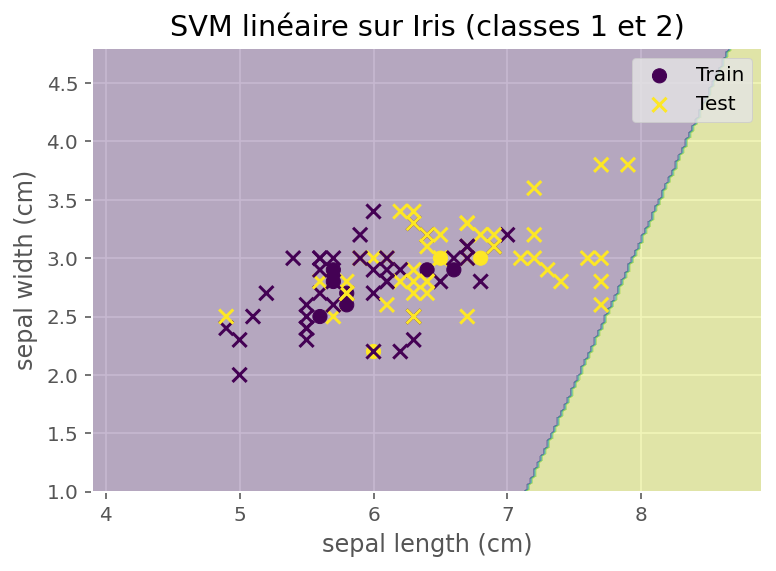
\includegraphics[width=0.8\textwidth]{vis/classif_90test_10train.png}
    \caption{SVM linéaire avec 90\% des données réservées au test}
    \label{fig:svm_iris_90test_10train}
\end{figure}

Ci-dessus, on a dédiées 90\% des données pour le test, ce qui ne laisse
qu'environ 10\% pour l'entraînement (soit seulement 10 points). Avec si
peu d'exemples, le SVM ne dispose pas d'assez d'informations pour bien
apprendre. On a alors que la frontière de décision est très
approximative et la précision sur le test chute à \textbf{0.48}, proche
du hasard.

En utilisant 40\% des données pour le test, nous obtenons une précision
de 7\%. Comparée à la \textbf{figure 1}, la frontière de décision sépare
mieux les points, bien que quelques erreurs de prédiction subsistent. La
\textbf{figure 2} ci-dessous illustre cette visualisation.

\begin{figure}[H]
    \centering
    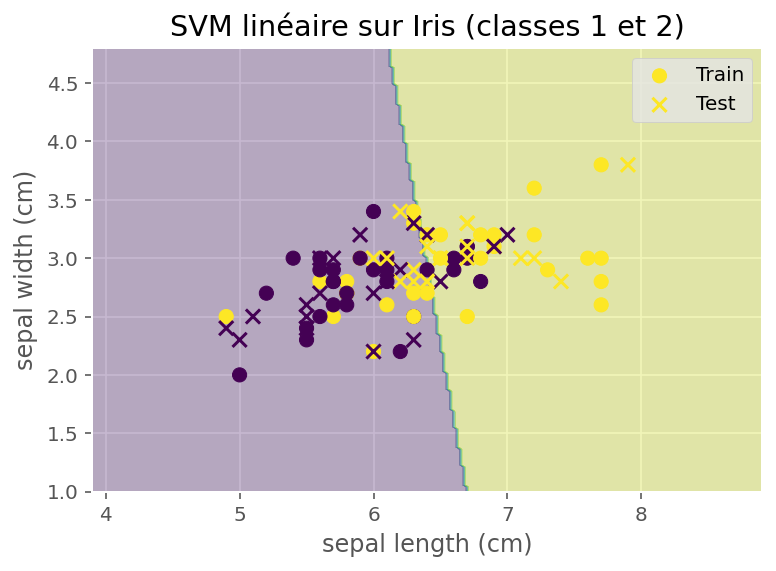
\includegraphics[width=0.65\textwidth]{vis/classif_40test_60train.png}
    \caption{SVM linéaire avec 40\% des données réservées au test}
    \label{fig:svm_iris_40test_60train}
\end{figure}

\subsection{\texorpdfstring{\textcolor{blue}{2.2. SVM polynomial : discrimination entre les classes 1 et 2 d’Iris}}{}}\label{section-3}

Dans cette section, nous entraînons un SVM avec noyau polynomial pour
discriminer les classes 1 et 2 d'Iris. Ce noyau permet de modéliser des
frontières de décision non linéaires, plus flexibles que celles du SVM
linéaire. Nous comparerons ensuite ses performances et sa frontière de
décision avec celles du SVM linéaire présenté précédemment.

\begin{figure}[H]
    \centering
    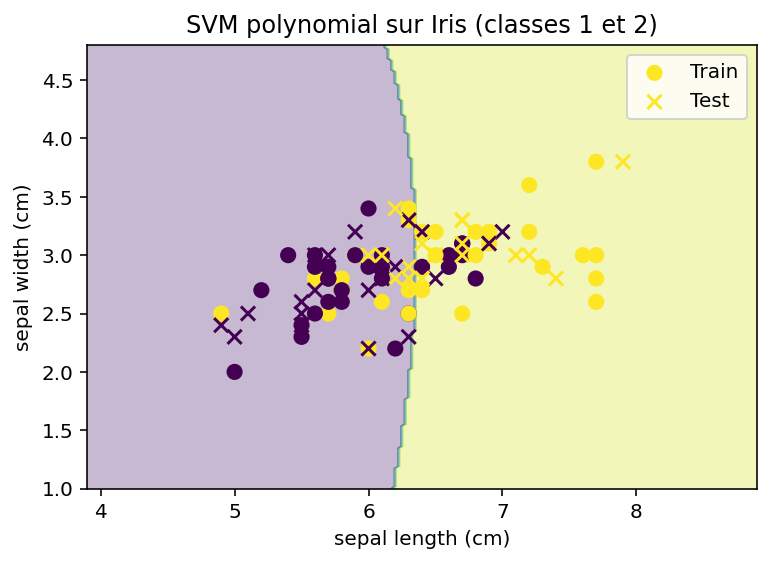
\includegraphics[width=0.65\textwidth]{vis/classif_poly_40test_60train.png}
    \caption{SVM polynomial avec 40\% des données réservées au test}
    \label{fig:svm_poly_iris_40test_60train}
\end{figure}

À présent, nous comparons la classification linéaire à la classification
polynomiale. Cette dernière ajuste mieux la frontière de décision, avec
une précision de 0.75 sur le jeu de test. Comme pour la classification
linéaire, 40\% des données ont été utilisées pour l'évaluation.

\begin{figure}[H]
    \centering
    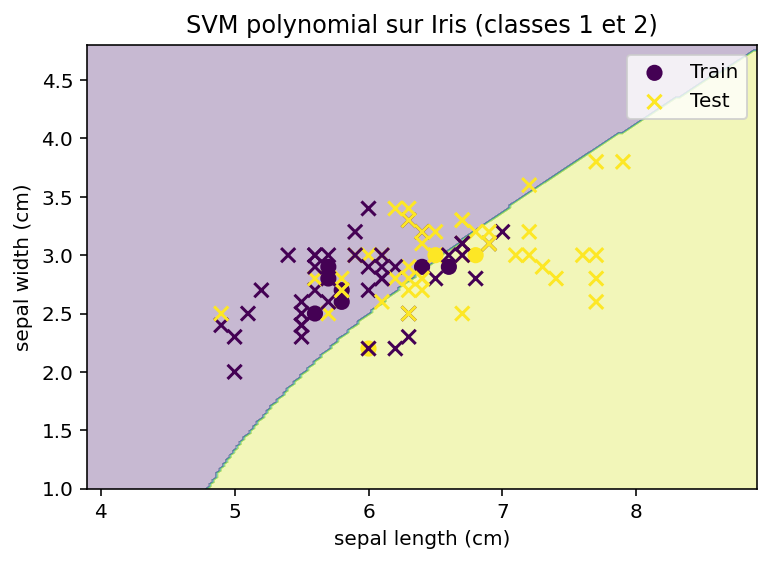
\includegraphics[width=0.65\textwidth]{vis/classif_poly_90test_10train.png}
    \caption{SVM polynomial avec 90\% des données réservées au test}
    \label{fig:svm_poly_iris_90test_10train}
\end{figure}

Nous avons testé deux modèles SVM (linéaire et polynomial) sur les
classes 1 et 2 de l'iris, en utilisant les caractéristiques
\textit{sepal length} et \textit{sepal width}.

Avec une grande proportion de données en test (90\%), les deux modèles
donnent de faibles scores, mais le SVM polynomial s'adapte mieux grâce à
une frontière de décision non linéaire.

Avec une répartition plus équilibrée (60\% train / 40\% test), les
performances s'améliorent. Le SVM polynomial reste légèrement meilleur,
car il capture mieux la séparation non linéaire entre les classes.

\subsection{\texorpdfstring{\textcolor{blue}{2.3. SVM GUI: données simulées déséquilibré}}{}}\label{section-4}

Cette application
\textcolor{red}{svm\_gui.py}(\textcolor{blue}{https://scikit-learn.org/1.2/auto\_examples/applications/svm\_gui.html})
permet en temps réel d'évaluer l'impact du noyaux et du paramètre de
régularisation \(C\).

Dans ce qui suit, nous allons générer un jeu de données très
déséquilibré avec beaucoup plus de points dans une classe que dans
l'autre. Ensuite, nous utiliserons un noyau linéaire tout en réduisant
le paramètre \(C\) et observerons le résultat.

Lorsque l'on diminue la valeur du paramètre \(C=0,001\), le SVM devient
plus tolérant aux erreurs. La frontière de décision se simplifie et ne
cherche plus à bien séparer toutes les classes.

Dans un jeu de données très déséquilibré (90\% vs 10\%), cela entraîne
un fort biais vers la classe majoritaire. La classe minoritaire est
alors mal reconnue, voire ignorée. La figure ci-dessous illustre la
frontière de décision d'un problème déséquilibré:

\begin{figure}[H]
    \centering
    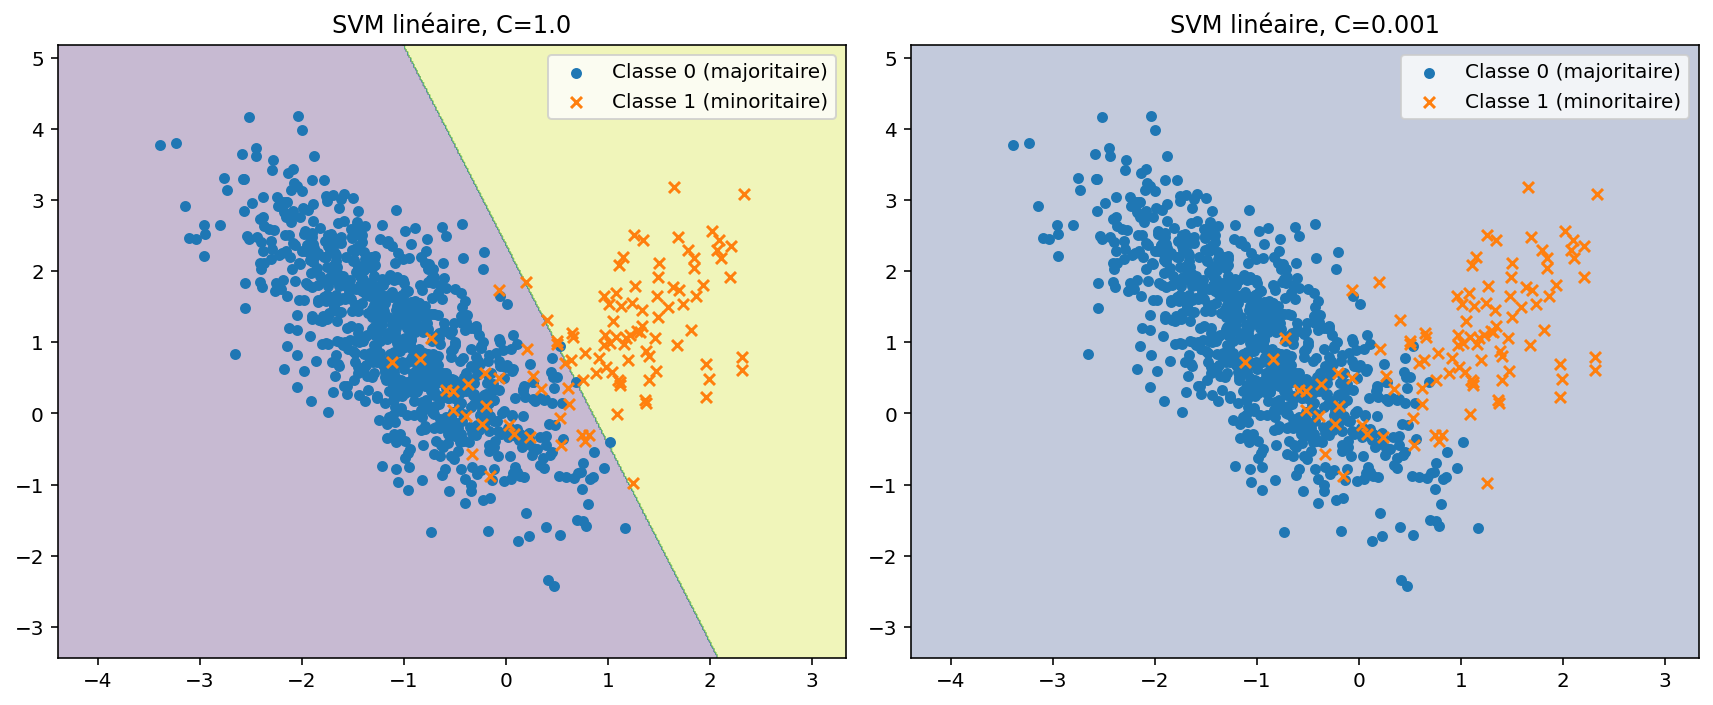
\includegraphics[width=0.9\textwidth]{vis/classif_simul_cpetit.png}
    \caption{SVM linéaire avec $C = 0.001$ sur données déséquilibrées.}
    \label{fig:simule_c_petit}
\end{figure}

Pour résoudre le problème de données déséquilibrées, nous pouvons
utiliser l'option \texttt{class\_weight="balanced"} dans le SVM. Cette
approche permet d'ajouter une correction par pondération, en donnant
davantage de poids à la classe minoritaire afin d'éviter qu'elle soit
ignorée par le modèle.

L'illustration de ce phénomène, avec et sans correction par pondération,
est présentée en annexe.

\section{\texorpdfstring{\textcolor{red}{3. Classification de visage}}{}}\label{section-5}

Dans cette partie, nous allons étudier un problème de classification
appliqué à des visages.\\
La base de données utilisée est disponible à l'adresse suivante :\\
\textcolor{blue}{\url{https://github.com/atttoum8643f/tp_svm/tree/main/data/olivetti_visages}}.

L'objectif est d'entraîner un SVM afin de distinguer différents
individus, et d'analyser l'impact du paramètre de régularisation \(C\)
sur les performances du modèle.

\subsection{\texorpdfstring{\textcolor{blue}{3.1. Évaluation de l’influence du paramètre $C$}}{}}\label{section-6}

La figure ci-dessous illustre l'évolution de l'erreur de prédiction en
fonction du paramètre de régularisation \(C\) dans un SVM linéaire.\\
Pour des valeurs très faibles (\(C \leq 10^{-4}\)), l'erreur est élevée
(autour de 45--60\%), ce qui traduit un modèle trop régularisé et
sous-apprenant.\\
À partir de \(C \approx 10^{-3}\), l'erreur chute fortement et atteint
environ 15\%.\\
Ensuite, pour des valeurs plus grandes de \(C\) (entre \(10^{-2}\) et
\(10^{5}\)), l'erreur se stabilise, indiquant que l'augmentation de
\(C\) n'apporte plus de gain significatif.

\begin{figure}[H]
    \centering
    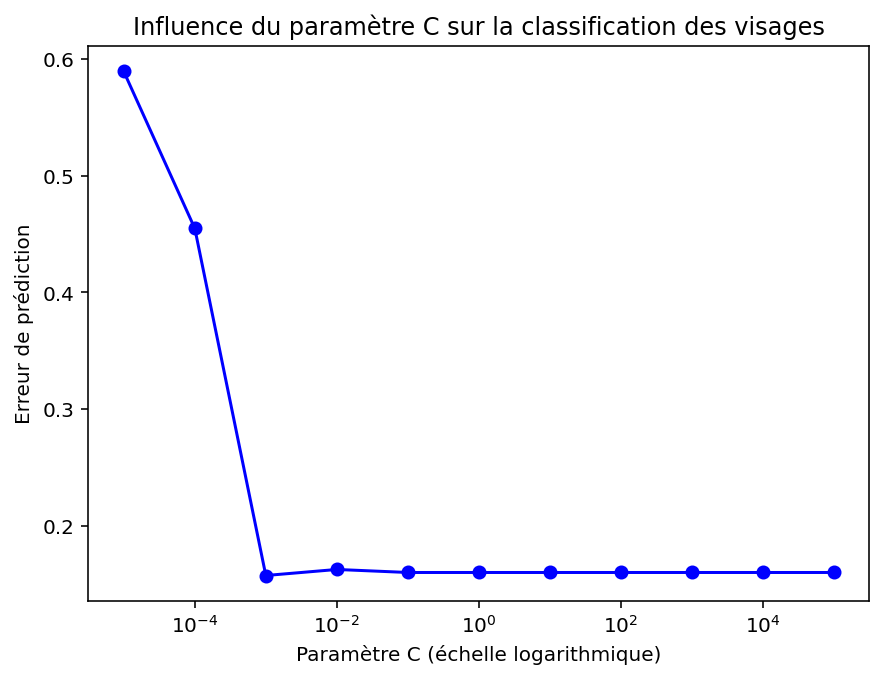
\includegraphics[width=0.6\textwidth]{vis/influence_c.png}
    \caption{Influence du paramètre C sur la classification de visages}
    \label{fig:influence_de_c}
\end{figure}

L'introduction de variables parasites dégrade la qualité de la
classification. En effet, les résultats obtenus mettent en évidence
l'impact des variables de nuisance sur les performances du
classifieur.\\
Sans ajout de bruit, le taux d'erreur est d'environ \(0.152\), soit une
précision proche de \(85\%\).\\
En revanche, lorsque l'on ajoute \(500\) variables de nuisance, l'erreur
augmente à \(0196\) (soit une précision d'environ \(80\%\)).

Néanmoins, le SVM reste relativement robuste puisque la performance
globale demeure correcte (voir la fonction \textbf{erreur\_svm} se
trouvant dans \textbf{influ\_erreur\_c.py}).

\subsection{\texorpdfstring{\textcolor{blue}{3.2. Amélioration de la prédiction via un ACP}}{}}\label{section-7}

Afin d'améliorer les performances du classifieur, nous utilisons une
réduction de dimension par \textit{Analyse en Composantes Principales}
(ACP), implémentée dans \texttt{sklearn.decomposition.PCA} avec l'option
\texttt{svd\_solver='randomized'}.

L'ACP avec le critère de Kaiser (\textbf{garder que les composantes qui
ont des valeurs propres supérieures à un}) a permis de réduire fortement
la dimension des données : on passe de
\textbf{1850 variables initiales à seulement 137 composantes principales}.
Cela correspond à une réduction de plus de \textbf{90\%} de la
dimension.

Malgré cette réduction importante, le modèle conserve une
\textbf{bonne précision (0.770)} et explique une grande partie de
l'information contenue dans les données, avec une
\textbf{inertie expliquée de 93.9\%}.

En d'autres termes, on simplifie fortement les données tout en gardant
l'essentiel de leur structure et de leur pouvoir explicatif.

\begin{figure}[H]
    \centering
    % Première image
    \begin{minipage}{0.48\textwidth}
        \centering
        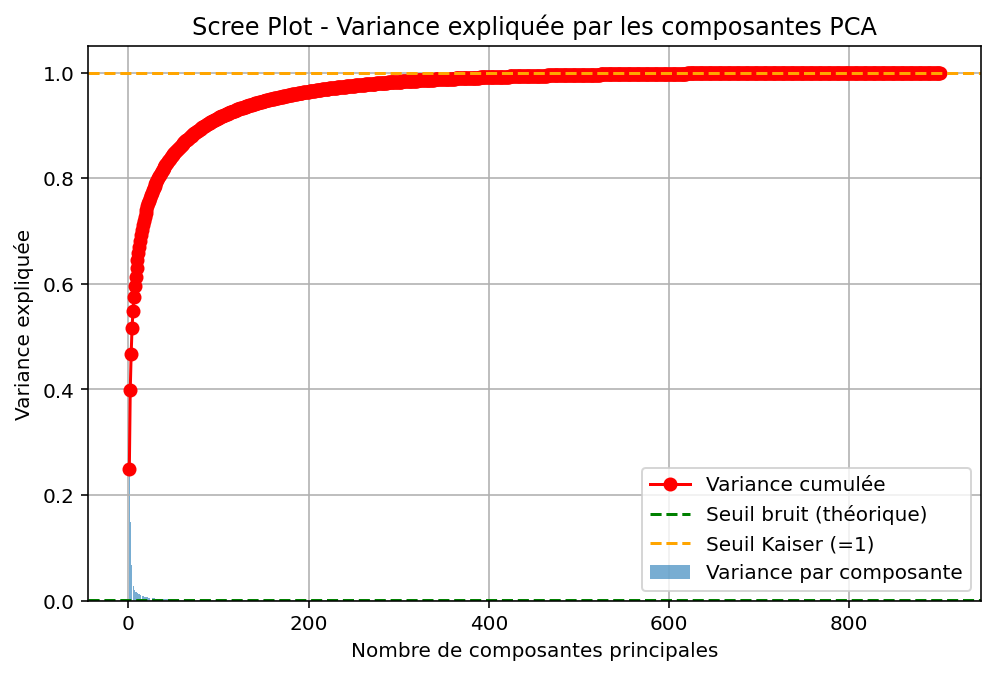
\includegraphics[width=\linewidth]{vis/variance_exp.png}
        \caption{Variance expliquée}
        \label{fig:variance_exp}
    \end{minipage}
    \hfill
    % Deuxième image
    \begin{minipage}{0.48\textwidth}
        \centering
        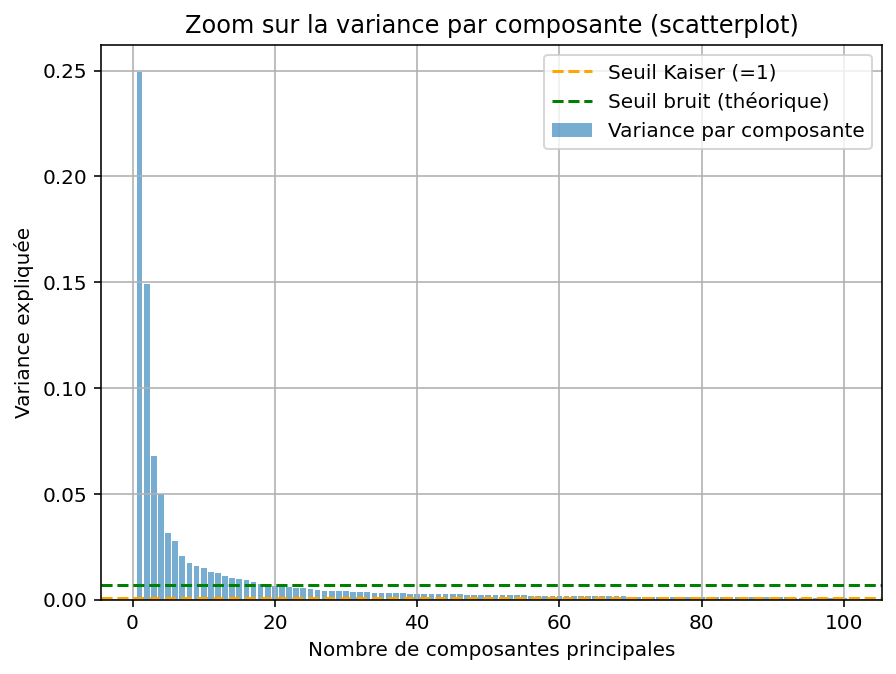
\includegraphics[width=\linewidth]{vis/scatterplot_cp.png}
        \caption{Scatter plot des composantes}
        \label{fig:scatterplot_cp}
    \end{minipage}
    \label{fig:pca_results}
\end{figure}

Il existe un biais dans notre prétraittement des données de
\textbf{svm\_script.py}, en effet, la normalisation (centrage-réduction)
est appliquée \textbf{avant} la séparation entre les ensembles
d'apprentissage et de test.

\begin{Shaded}
\begin{Highlighting}[]
\CommentTok{\# Scale features (lignes 224–226)}
\NormalTok{X }\OperatorTok{{-}=}\NormalTok{ np.mean(X, axis}\OperatorTok{=}\DecValTok{0}\NormalTok{)}
\NormalTok{X }\OperatorTok{/=}\NormalTok{ np.std(X, axis}\OperatorTok{=}\DecValTok{0}\NormalTok{)}

\CommentTok{\# Split data into a half training and half test set}
\CommentTok{\# X\_train, X\_test, y\_train, y\_test, images\_train, images\_test = \textbackslash{}}
\CommentTok{\#    train\_test\_split(X, y, images, test\_size=0.5, random\_state=0)}
\CommentTok{\# X\_train, X\_test, y\_train, y\_test = \textbackslash{}}
\CommentTok{\#    train\_test\_split(X, y, test\_size=0.5, random\_state=0)}
\end{Highlighting}
\end{Shaded}

Ici, la moyenne et l'écart-type sont calculés sur toutes les données
(train + test confondus), ce qui introduit une fuite d'information. La
normalisation doit être faite après le split, en utilisant uniquement
les statistiques de l'ensemble d'apprentissage.

\newpage

\section{\texorpdfstring{\textcolor{red}{4. Annexe}}{}}\label{section-8}

Ce code génère un jeu de données binaire fortement déséquilibré (90,\%
vs 10,\%). Deux modèles SVM linéaires sont ensuite entraînés : l'un sans
pondération et l'autre avec l'option \texttt{class\_weight="balanced"}.
Enfin, la frontière de décision de chaque modèle est tracée afin de
comparer l'effet de la pondération sur la classe minoritaire.

Le code complet utilisé pour générer les comparaisons de frontières de
décision est disponible sur GitHub à l'adresse suivante :

\textcolor{blue}{\url{https://github.com/atttoum8643f/tp_svm/blob/main/code_py/corr_ponderation.py}}

\begin{figure}[H]
    \centering
    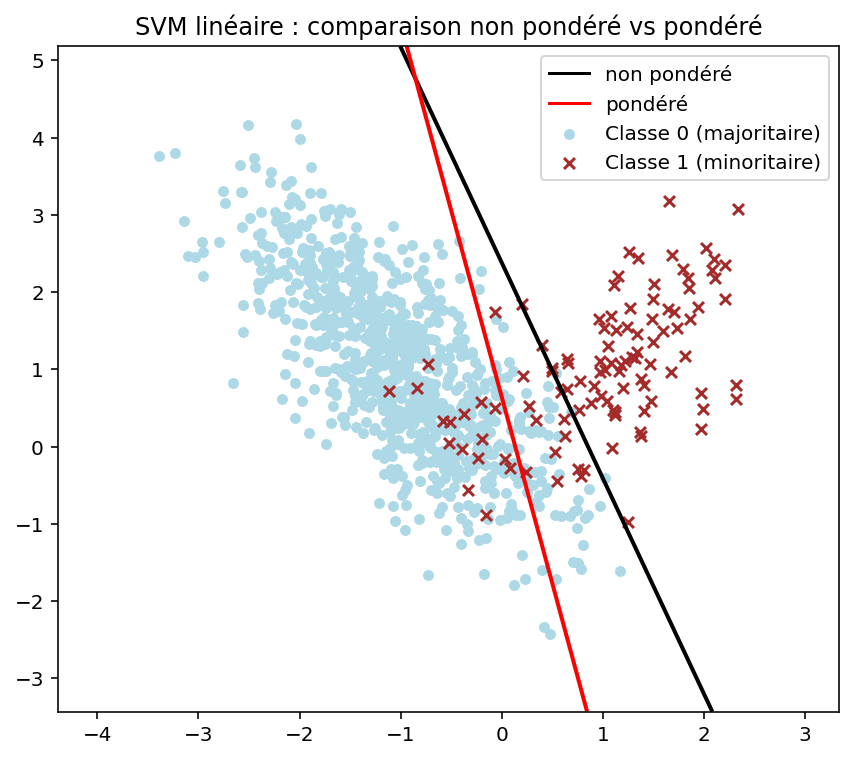
\includegraphics[width=0.75\textwidth]{vis/pond.png}
    \caption{Frontière de décision d’un SVM linéaire avec et sans correction par pondération}
    \label{fig:avec_sans_pondération}
\end{figure}

\begin{thebibliography}{9}

\bibitem{scikit-learn}
scikit-learn developers.  
\textit{Support Vector Machines — scikit-learn documentation}.  
\url{http://scikit-learn.org/stable/modules/svm.html}.  
Consulté le 24 septembre 2025.

\bibitem{wiki-en}
Wikipedia.  
\textit{Support vector machine}.  
\url{http://en.wikipedia.org/wiki/Support_vector_machine}.  
Consulté le 24 septembre 2025.

\bibitem{wiki-fr}
Wikipédia.  
\textit{Machine à vecteurs de support}.  
\url{http://fr.wikipedia.org/wiki/Machine_%C3%A0_vecteurs_de_support}.  %C3%A0_vecteurs_de_support}.  %A0_vecteurs_de_support}.  
Consulté le 24 septembre 2025.

\end{thebibliography}

\end{document}
